\tikzset{every picture/.style={line width=0.75pt}} %set default line width to 0.75pt

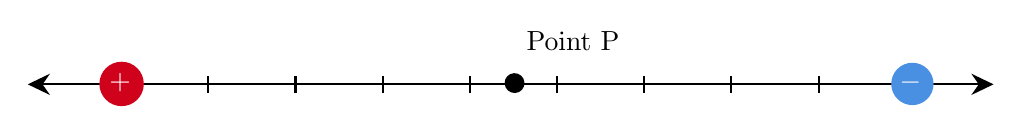
\begin{tikzpicture}[x=0.75pt,y=0.75pt,yscale=-1,xscale=1]
%uncomment if require: \path (0,300); %set diagram left start at 0, and has height of 300

%Straight Lines [id:da8648372319496271]
    \draw    (100,222) -- (559.3,222) (142,218) -- (142,226)(184,218) -- (184,226)(226,218) -- (226,226)(268,218) -- (268,226)(310,218) -- (310,226)(352,218) -- (352,226)(394,218) -- (394,226)(436,218) -- (436,226)(478,218) -- (478,226)(520,218) -- (520,226) ;
    \draw [shift={(562.3,222)}, rotate = 180] [fill={rgb, 255:red, 0; green, 0; blue, 0 }  ][line width=0.08]  [draw opacity=0] (10.72,-5.15) -- (0,0) -- (10.72,5.15) -- (7.12,0) -- cycle ;
    \draw [shift={(97,222)}, rotate = 0] [fill={rgb, 255:red, 0; green, 0; blue, 0 }  ][line width=0.08]  [draw opacity=0] (10.72,-5.15) -- (0,0) -- (10.72,5.15) -- (7.12,0) -- cycle ;
%Shape: Circle [id:dp525147663907922]
    \draw  [color={rgb, 255:red, 208; green, 2; blue, 27 }  ,draw opacity=1 ][fill={rgb, 255:red, 208; green, 2; blue, 27 }  ,fill opacity=1 ] (132,221.8) .. controls (132,216.17) and (136.57,211.6) .. (142.2,211.6) .. controls (147.83,211.6) and (152.4,216.17) .. (152.4,221.8) .. controls (152.4,227.43) and (147.83,232) .. (142.2,232) .. controls (136.57,232) and (132,227.43) .. (132,221.8) -- cycle ;
%Shape: Circle [id:dp6232351980171478]
    \draw  [draw opacity=0][fill={rgb, 255:red, 74; green, 144; blue, 226 }  ,fill opacity=1 ] (513,221.8) .. controls (513,216.17) and (517.57,211.6) .. (523.2,211.6) .. controls (528.83,211.6) and (533.4,216.17) .. (533.4,221.8) .. controls (533.4,227.43) and (528.83,232) .. (523.2,232) .. controls (517.57,232) and (513,227.43) .. (513,221.8) -- cycle ;
%Shape: Circle [id:dp8414250651719695]
    \draw  [fill={rgb, 255:red, 0; green, 0; blue, 0 }  ,fill opacity=1 ] (327.24,221.58) .. controls (327.11,219.22) and (328.92,217.22) .. (331.28,217.11) .. controls (333.64,217.01) and (335.67,218.84) .. (335.8,221.2) .. controls (335.93,223.56) and (334.13,225.56) .. (331.76,225.67) .. controls (329.4,225.77) and (327.38,223.94) .. (327.24,221.58) -- cycle ;

% Text Node
    \draw (134+.8,210+5) node [anchor=north west][inner sep=0.75pt]   [align=left] {\textcolor[rgb]{1,1,1}{+}};
% Text Node
    \draw (514+1.5,209+6) node [anchor=north west][inner sep=0.75pt]  [color={rgb, 255:red, 255; green, 255; blue, 255 }  ,opacity=1 ] [align=left] {$\displaystyle -$};
% Text Node
    \draw (335.8,195.2) node [anchor=north west][inner sep=0.75pt]   [align=left] {Point P};


\end{tikzpicture}
